\begin{figure*}[t]
    \centering
    \begin{subfigure}[b]{0.01\textwidth}
        \center
        \begin{turn}{90} 
            \scriptsize
            Average Returns
        \end{turn}
        \vspace{0.5cm}
    \end{subfigure}
    \begin{subfigure}[b]{0.27\textwidth}
        \center
        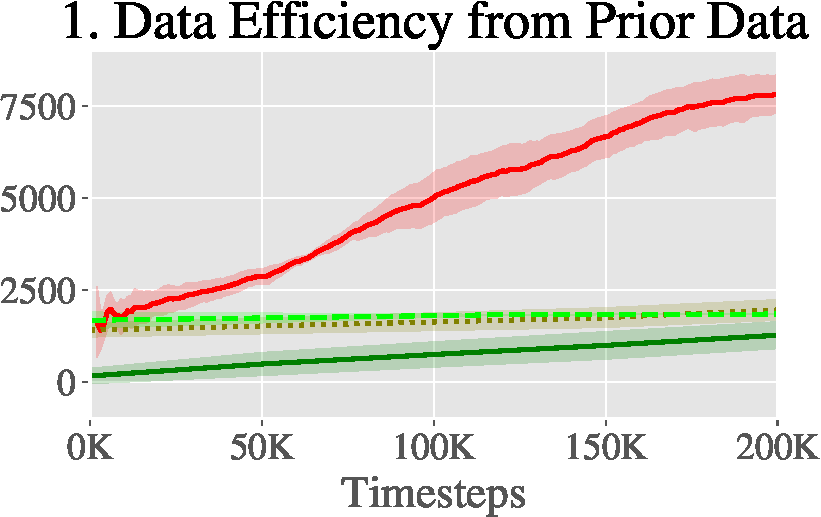
\includegraphics[height=2.2cm]{awac/figures/challenges/hc_pg-crop.pdf}
        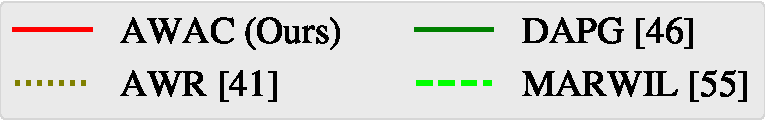
\includegraphics[height=0.55cm]{awac/figures/challenges/hc_pg_legend-crop.pdf}
    \end{subfigure}
    \begin{subfigure}[b]{0.25\textwidth}
        \center
        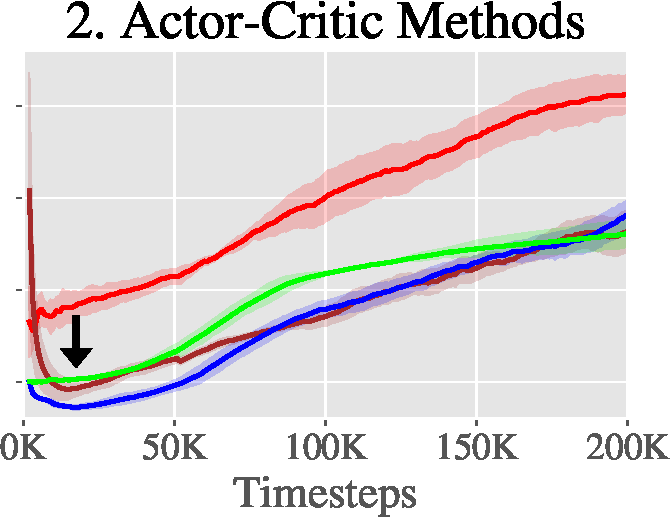
\includegraphics[height=2.2cm]{awac/figures/challenges/hc_sac-crop.pdf}
        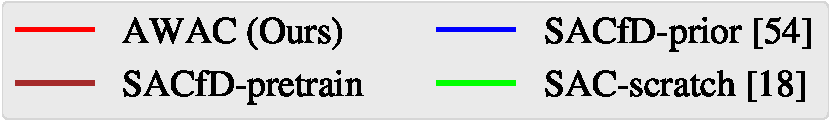
\includegraphics[height=0.55cm]{awac/figures/challenges/hc_sac_legend-crop.pdf}
    \end{subfigure}
    % \hfill
    \begin{subfigure}[b]{0.22\textwidth}
        \center
        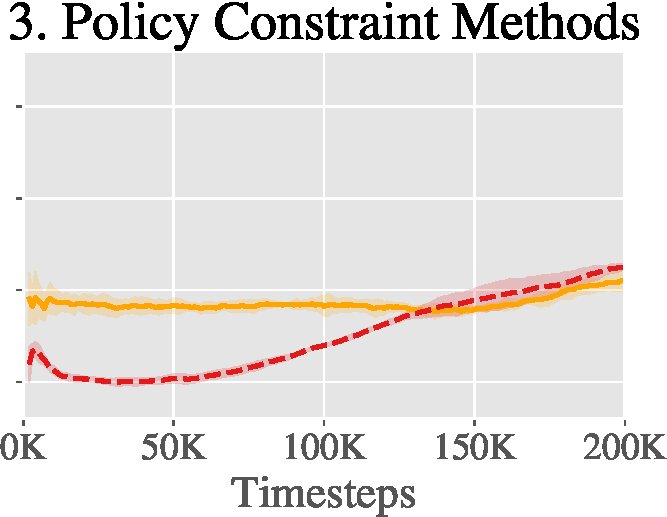
\includegraphics[height=2.2cm]{awac/figures/challenges/hc_constrain-crop.pdf}
        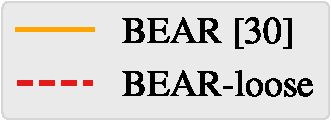
\includegraphics[height=0.55cm]{awac/figures/challenges/hc_constrain_legend-crop.pdf}
        % \vspace{0.23cm}
    \end{subfigure}
    \begin{subfigure}[b]{0.2\textwidth}
        \center
        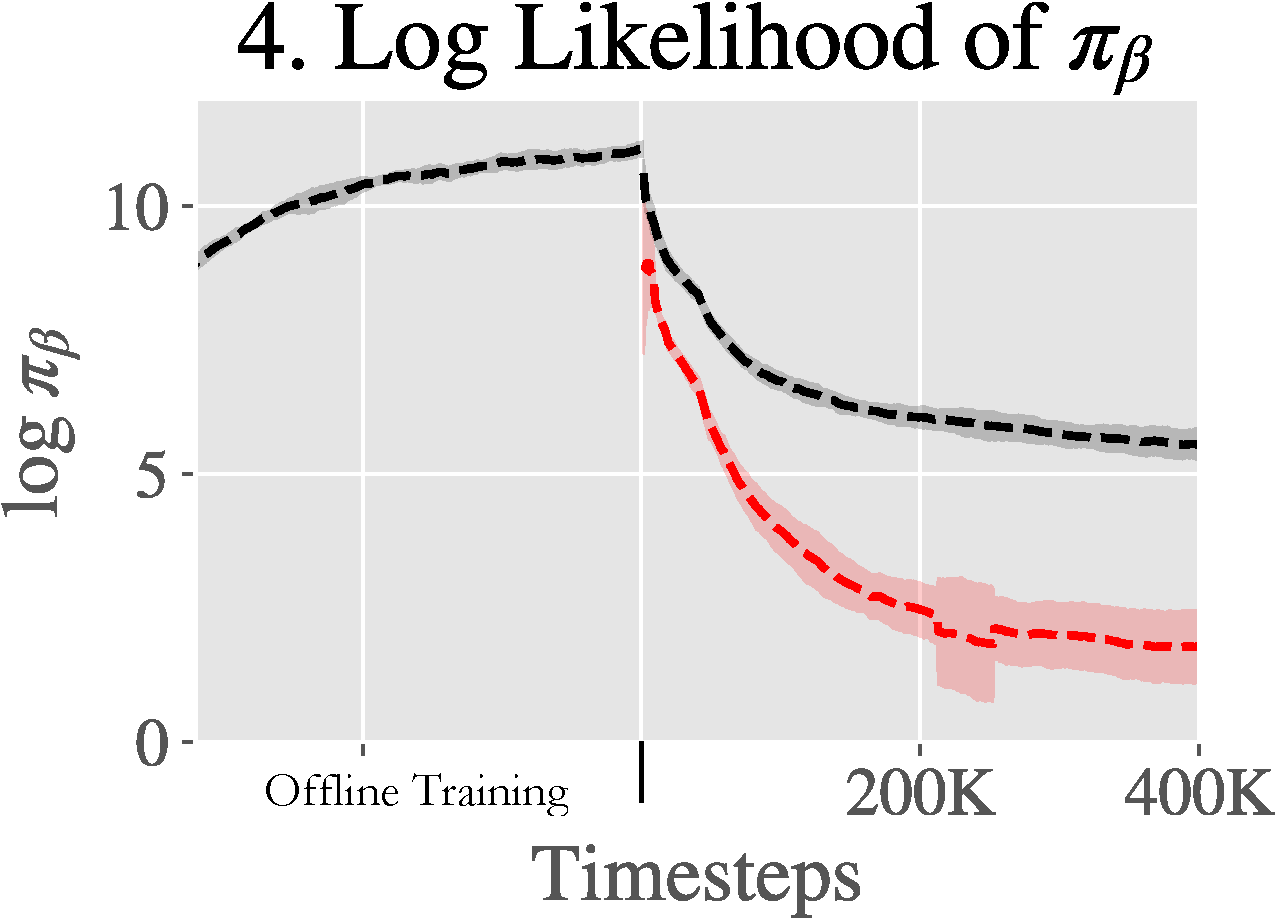
\includegraphics[height=2.2cm]{awac/figures/challenges/hc_logp_train-crop.pdf}
        \hspace{0.3cm}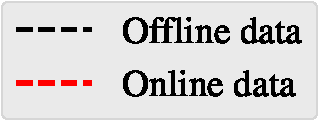
\includegraphics[height=0.55cm]{awac/figures/challenges/hc_log_probablation_legend-crop.pdf}
        % \vspace{1cm}
    \end{subfigure}
    
    \caption{
    % \small{
    Analysis of prior methods on HalfCheetah-v2 using offline RL with online fine-tuning. (1) On-policy methods (DAPG, AWR, MARWIL) 
    % ~\citep{rajeswaran2018dextrous} and AWR~\citep{peng2019awr} 
    learn relatively slowly, even with access to prior data. We present our method, AWAC, as an example of how off-policy RL methods can learn much faster. (2) Variants of soft actor-critic (SAC) with offline training (performed before timestep 0) and fine-tuning. We see a ``dip'' in the initial performance, even if the policy is pretrained with behavioral cloning.
    (3) Offline RL method BEAR~\citep{kumar19bear} on offline training and fine-tuning, including a ``loose'' variant of BEAR with a weakened constraint. Standard offline RL methods fine-tune slowly, while the ``loose'' BEAR variant experiences a similar dip as SAC. (4) We show that the fit of the behavior models $\hat{\pi}_\beta$ used by these offline methods
    degrades as new data is added to the buffer during fine-tuning, potentially explaining their poor fine-tuning performance.
    \vspace{-0.2in}
    % }
    % AWR \cite{peng2019awr} DAPG \cite{rajeswaran2018dextrous} MARWIL \cite{wang2018marwil} SACfD \cite{vecerik17ddpgfd} SAC \cite{haarnoja2018sac} BEAR \cite{kumar19bear}
    }
    \label{fig:challenges}
\end{figure*}